%%%%%%%%%%%%%%%%%%%%%%%%%%%%%%%%%%%%%%%%%
% Masters/Doctoral Thesis 
% LaTeX Template for IIITA Students
%
% Modified for:
% Token Optimisation: Cost-Efficient LLM Inference for Hindi-English Code-Mixed Task Prompts
%%%%%%%%%%%%%%%%%%%%%%%%%%%%%%%%%%%%%%%%%

%----------------------------------------------------------------------------------------
%	PACKAGES AND OTHER DOCUMENT CONFIGURATIONS
%----------------------------------------------------------------------------------------

\documentclass[
12pt, % The default document font size, options: 10pt, 11pt, 12pt
oneside, % Two side (alternating margins) for binding by default, uncomment to switch to one side
english, % ngerman for German
singlespacing, % options: singlespacing, onehalfspacing or doublespacing
liststotoc, % Add list of figures/tables/etc to table of contents
parskip, % Add space between paragraphs
headsepline, % Line under the header
]{Thesis} % The class file specifying the document structure

\usepackage{iftex}
\ifXeTeX
  % XeLaTeX has native UTF-8 and fontspec is loaded in Thesis.cls
  \usepackage{amssymb,amsfonts}
\else
  \usepackage[utf8]{inputenc}
  \usepackage[T1]{fontenc}
  \usepackage{mathpazo}
  \usepackage{amssymb,amsfonts}
\fi

\usepackage{tabularx}
\usepackage{subcaption}
\usepackage{listings}
\usepackage{xcolor}

\usepackage[backend=biber,
style=numeric,
bibencoding=utf8,
sorting=none
]{biblatex}
\addbibresource{example.bib} % The filename of the bibliography
\usepackage[autostyle=true]{csquotes} % Required to generate language-dependent quotes
\usepackage{array}

% Code snippet styling
\definecolor{codegreen}{rgb}{0,0.6,0}
\definecolor{codegray}{rgb}{0.5,0.5,0.5}
\definecolor{codepurple}{rgb}{0.58,0,0.82}
\definecolor{backcolour}{rgb}{0.96,0.96,0.96}

\lstdefinestyle{mystyle}{
    backgroundcolor=\color{backcolour},   
    commentstyle=\color{codegreen},
    keywordstyle=\color{blue},
    numberstyle=\tiny\color{codegray},
    stringstyle=\color{codepurple},
    basicstyle=\ttfamily\footnotesize,
    breakatwhitespace=false,         
    breaklines=true,                 
    captionpos=b,                    
    keepspaces=true,                 
    numbers=left,                    
    numbersep=5pt,                  
    showspaces=false,                
    showstringspaces=false,
    showtabs=false,                  
    tabsize=2
}
\lstset{style=mystyle}

%----------------------------------------------------------------------------------------
%	MARGIN SETTINGS
%----------------------------------------------------------------------------------------

\geometry{
	paper=a4paper,
	inner=20mm,
	outer=20mm,
	bindingoffset=5mm,
	top=25mm,
	bottom=20mm,
}

%----------------------------------------------------------------------------------------
%	THESIS DETAILS & STUDENT CONFIGURATION
%----------------------------------------------------------------------------------------

\thesistitle{Token Optimisation: Cost-Efficient LLM Inference for Hindi-English Code-Mixed Task Prompts}
\degree{Bachelor of Technology}

% SUPERVISOR DETAILS
\supervisor{Dr. Sonali Agrawal}

% STUDENT DETAILS
\newcommand{\studentonename}{Tushar Saharan}
\newcommand{\studentoneroll}{IIT2021001}

\newcommand{\studenttwoname}{Shivam Kumar}
\newcommand{\studenttworoll}{IIT2021002}

\newcommand{\studentthreename}{Sahil Gupta}
\newcommand{\studentthreeroll}{IIT2021003}

% DEPARTMENT & UNIVERSITY
\department{Department of Information Technology}
\university{Indian Institute of Information Technology, Allahabad}
\subject{Information Technology}

% Helper formatting commands
\newcommand{\studentnamesformatted}{%
\studentonename%
\ifdefined\studenttwoname%
\\\studenttwoname%
\fi%
\ifdefined\studentthreename%
\\\studentthreename%
\fi%
}

\newcommand{\rollnumbersformatted}{%
\studentoneroll%
\ifdefined\studenttworoll%
\\\studenttworoll%
\fi%
\ifdefined\studentthreeroll%
\\\studentthreeroll%
\fi%
}

\newcommand{\studentnamescomma}{%
\studentonename%
\ifdefined\studenttwoname%
, \studenttwoname%
\fi%
\ifdefined\studentthreename%
, \studentthreename%
\fi%
}

\newcommand{\studentnamesdeclaration}{%
\studentonename{} (\studentoneroll)%
\ifdefined\studenttwoname%
, \studenttwoname{} (\studenttworoll)%
\fi%
\ifdefined\studentthreename%
, and \studentthreename{} (\studentthreeroll)%
\fi%
}

\newcommand{\studentsignatures}{%
\studentonename{} (\studentoneroll)%
\ifdefined\studenttwoname%
\\\studenttwoname{} (\studenttworoll)%
\fi%
\ifdefined\studentthreename%
\\\studentthreename{} (\studentthreeroll)%
\fi%
}

\newcommand{\pronounwe}{%
\ifdefined\studenttwoname%
We%
\else%
I%
\fi%
}

\newcommand{\pronounus}{%
\ifdefined\studenttwoname%
us%
\else%
me%
\fi%
}

\firstauthor{\studentnamesformatted}
\enrollmentnumber{\rollnumbersformatted}

\examiner{} 
\addresses{} 
\keywords{Prompt Compression, Code-Mixing, Hinglish, Cascade Routing, Conformal Prediction, Inference Economics, Tokenizer Tax} 
\faculty{Faculty of Information Technology}

\AtBeginDocument{
\hypersetup{pdftitle=\ttitle}
\hypersetup{pdfkeywords=\keywordnames}
}

\begin{document}
\begin{sloppypar}

%----------------------------------------------------------------------------------------
%	FRONT MATTER
%----------------------------------------------------------------------------------------

\frontmatter % Use roman page numbering style (i, ii, iii, iv...) for the pre-content pages

\pagestyle{plain} 

%----------------------------------------------------------------------------------------
%	TITLE PAGE
%----------------------------------------------------------------------------------------

\begin{titlepage}
\begin{center}
\begin{spacing}{1.2}

{\huge \bfseries \ttitle\par}

\vspace{5mm}
\textit{A thesis submitted in partial fulfillment of the requirements\\for the award of the degree of} 

\vspace{7mm}
\textsc{\huge \MakeUppercase{\degreename}}

\vspace{3mm}

\includegraphics[width=5cm]{Figures/IIITA_Logo.png}
\vspace{5mm}

\begin{minipage}[t]{0.5\textwidth}
    \begin{flushleft} \large
        \textit{By:-} \\
        \textsc{\studentnamesformatted}
    \end{flushleft}
\end{minipage}
\begin{minipage}[t]{0.45\textwidth}
    \begin{flushright} \large
        \textit{Enrollment No.} \\
        \textsc{\rollnumbersformatted}
    \end{flushright}
\end{minipage}\\[1cm]

\textit{Under the Supervision of}\\[2mm]
\textsc{\Large \supname}\\
\vspace{7mm}
\textit{Submitted to the}\\[2mm]
\textsc{\Large \deptname}\\

\vspace{12mm}
\ifdefined\devanagarifont
\begin{hindi}
    {\Large\textbf{भारतीय सूचना प्रौद्योगिकी संस्थान, इलाहाबाद}}
\end{hindi} \\[3mm]
\else
{\Large\textbf{भारतीय सूचना प्रौद्योगिकी संस्थान, इलाहाबाद}}\\[3mm]
\fi
\textsc{\Large \univname}

\vspace{5mm}
\monthyear

\end{spacing}
\end{center}
\end{titlepage}

%----------------------------------------------------------------------------------------
%	CERTIFICATE
%----------------------------------------------------------------------------------------
\checktoopen
\begin{figure}[htp]
    
\includegraphics[height=2.8cm,keepaspectratio]{Figures/IIITA_Header.png}
\end{figure}
\thispagestyle{empty}

\begin{spacing}{1.5}
\begin{center}
    {\centering\large\bfseries CERTIFICATE \par\vspace{10pt}}
\end{center}

\noindent It is certified that the work contained in the thesis titled \enquote{\ttitle} by {\studentnamescomma} has been carried out under my supervision and that this work has not been submitted elsewhere for a degree.

\vspace{3cm}
\hfill\begin{minipage}{7.5cm}
    \begin{spacing}{1.2}
        \par
        \rule{\textwidth}{0.2pt}\\
        {\supname} \par
        {\deptname} \par
        IIIT Allahabad \par
    \end{spacing}
\end{minipage}

\end{spacing}
\cleardoublepage

%----------------------------------------------------------------------------------------
%	CANDIDATE DECLARATION
%----------------------------------------------------------------------------------------
\checktoopen
\begin{figure}[htp]
    
\includegraphics[height=2.8cm,keepaspectratio]{Figures/IIITA_Header.png}
\end{figure}
\thispagestyle{empty}
\vspace{1mm}

\begin{center}
    {\large\bfseries CANDIDATE DECLARATION}
\end{center}

\begin{spacing}{1.2}

\noindent \pronounwe, \studentnamesdeclaration, hereby certify that the thesis titled \enquote{\ttitle} has been submitted by \pronounus{} in partial fulfillment of the requirements for the Degree of \degreename{} in the \deptname{} at the \univname.

\par
\noindent We acknowledge that plagiarism includes: 
\begin{enumerate} 
    \item Reproducing another person's work (fully or partially) or ideas and presenting them as our own.
    \item Copying or paraphrasing another person's work without appropriate attribution.
    \item Engaging in literary theft by reproducing a unique literary construct without crediting its source.
\end{enumerate}
\par
We affirm that due credit has been given to all original authors and sources through proper citations for words, ideas, diagrams, graphics, computer programs, experiments, results, and websites that are not our own contributions. Direct quotations have been appropriately marked, and sources have been properly referenced. Furthermore, we declare that no portion of our work is plagiarized. In the event of a plagiarism claim, we accept full responsibility for the contents of this thesis. We acknowledge that our supervisor may not be able to verify the originality of every aspect of our work.
\end{spacing}

\begin{spacing}{2.0}
\noindent
\begin{minipage}[t]{0.4\textwidth}  
    \begin{flushleft} 
        Place: Prayagraj\\
    \end{flushleft}
\end{minipage}
\hfill
\begin{minipage}[t]{0.4\textwidth}  
    \begin{flushright}         
        Date: \rule{40mm}{0.1pt}\\       
    \end{flushright}
\end{minipage}
\par
{\studentsignatures}
\end{spacing}

\cleardoublepage

%----------------------------------------------------------------------------------------
%	ABSTRACT PAGE
%----------------------------------------------------------------------------------------

\begin{abstract}
\begin{spacing}{1.5}

\addchaptertocentry{\abstractname}

Large Language Model (LLM) serving costs scale directly with prompt token count and selected model tier. While prompt compression reduces costs on clean English corpora, standard subword tokenizers (e.g., Byte-Pair Encoding) severely over-segment Hindi-English (Hinglish) code-mixed text, imposing an implicit 2.1$\times$ \textit{Tokenizer Tax} on multilingual users. Furthermore, naive neural compressors mangle named entities, numerical values, and transliterated syntax, dropping downstream task completion.

In this thesis, we design, implement, and empirically validate an OpenAI-compatible 12-module serving gateway that jointly optimizes prompt length and model selection for code-mixed dialogue. Our architecture couples a 5-stage CPU-efficient prompt compressor with a conformal cascade router. The compressor introduces consonant-skeleton phonetic hashing to collapse spelling entropy, heuristic filler stripping, force-preserved regex safety masking, and a 25-feature Linear-Chain Conditional Random Field (CRF) sequence tagger operating in under 10\,ms without GPU overhead. The cascade router employs a fine-tuned ModernBERT-large difficulty classifier calibrated via Hoeffding Learn-Then-Test (LTT) risk bounds to dispatch simple queries to cost-efficient 8B models while routing complex reasoning to frontier 120B models under a provable statistical error budget ($\alpha = 0.05$).

Evaluated across 5,804 task-oriented dialogue rows from the PRESTO benchmark and 3,000 code-mixed queries, our protected-span mechanism achieves exactly 1.000 entity recall across 680 dialogue rows, eliminating the 20--31\% entity mangling observed in raw baselines. In addition, the gateway reduces metered token intake by 38.3--47.6\% and cuts inference costs by over 60\% without degrading downstream task success. All modules, benchmarks, and interactive audit receipt tools are open-sourced to promote equitable NLP serving in low-resource and code-mixed settings.

\end{spacing}
\end{abstract}

%----------------------------------------------------------------------------------------
%	ACKNOWLEDGEMENTS
%----------------------------------------------------------------------------------------

\begin{acknowledgements}
\begin{spacing}{1.5}
\addchaptertocentry{\acknowledgementname}

We would like to express our deepest gratitude to our project supervisor, \textbf{Dr. Sonali Agrawal}, Department of Information Technology, Indian Institute of Information Technology, Allahabad, for her constant guidance, constructive critique, and invaluable encouragement throughout this research. Her high standards for empirical rigor and methodological discipline shaped the direction and execution of this work.

We extend our sincere thanks to the faculty members and staff of the Department of Information Technology for providing the institutional support, computational infrastructure, and academic environment essential for completing this project.

We are also thankful to our peers and lab colleagues for engaging discussions, review feedback, and collaborative testing of our gateway system. Lastly, we owe heartfelt gratitude to our parents and families for their unwavering patience, support, and sacrifices that enabled our academic journey.

\vspace{1cm}
\begin{flushright}
\textit{Tushar Saharan}\\
\textit{Shivam Kumar}\\
\textit{Sahil Gupta}
\end{flushright}

\end{spacing}
\end{acknowledgements}

%----------------------------------------------------------------------------------------
%	LIST OF CONTENTS/FIGURES/TABLES PAGES
%----------------------------------------------------------------------------------------

\tableofcontents

\listoffigures

\listoftables

%----------------------------------------------------------------------------------------
%	ABBREVIATIONS
%----------------------------------------------------------------------------------------

\begin{abbreviations}{ll}

\textbf{API}  & \textbf{A}pplication \textbf{P}rogramming \textbf{I}nterface \\
\textbf{BERT} & \textbf{B}idirectional \textbf{E}ncoder \textbf{R}epresentations from \textbf{T}ransformers \\
\textbf{BLEU} & \textbf{B}i\textbf{L}ingual \textbf{E}valuation \textbf{U}nderstudy \\
\textbf{BPE}  & \textbf{B}yte \textbf{P}air \textbf{E}ncoding \\
\textbf{CI}   & \textbf{C}onfidence \textbf{I}nterval \\
\textbf{CRF}  & \textbf{C}onditional \textbf{R}andom \textbf{F}ield \\
\textbf{ECE}  & \textbf{E}xpected \textbf{C}alibration \textbf{E}rror \\
\textbf{EM}   & \textbf{E}xact \textbf{M}atch \\
\textbf{GPU}  & \textbf{G}raphics \textbf{P}rocessing \textbf{U}nit \\
\textbf{GRPO} & \textbf{G}roup \textbf{R}elative \textbf{P}olicy \textbf{O}ptimization \\
\textbf{LLM}  & \textbf{L}arge \textbf{L}anguage \textbf{M}odel \\
\textbf{LPU}  & \textbf{L}anguage \textbf{P}rocessing \textbf{U}nit \\
\textbf{LTT}  & \textbf{L}earn-\textbf{T}hen-\textbf{T}est \\
\textbf{MuRIL}& \textbf{Mu}ltilingual \textbf{R}epresentations for \textbf{I}ndian \textbf{L}anguages \\
\textbf{NER}  & \textbf{N}amed \textbf{E}ntity \textbf{R}ecognition \\
\textbf{NLP}  & \textbf{N}atural \textbf{L}anguage \textbf{P}rocessing \\
\textbf{ROUGE}& \textbf{R}ecall-\textbf{O}riented \textbf{U}nderstudy for \textbf{G}isting \textbf{E}valuation \\
\textbf{SSE}  & \textbf{S}erver-\textbf{S}ent \textbf{E}vents \\
\textbf{UCB}  & \textbf{U}pper \textbf{C}onfidence \textbf{B}ound \\

\end{abbreviations}

%----------------------------------------------------------------------------------------
%	DEDICATION
%----------------------------------------------------------------------------------------

\dedicatory{Dedicated to our families, teachers, and the open-source NLP research community.}


%----------------------------------------------------------------------------------------
%	THESIS CONTENT - CHAPTERS
%----------------------------------------------------------------------------------------

\mainmatter % Begin numeric (1,2,3...) page numbering

\pagestyle{thesis} % Return the page headers back to the "thesis" style
\begin{spacing}{1.5}

% Chapter 1: Introduction

\chapter{Introduction}
\label{chap:introduction}

\section{Background and Motivation}
Large Language Models (LLMs) have emerged as the foundational substrate for contemporary natural language processing, powering applications spanning customer support, autonomous coding, personal productivity, and dialogue-driven interfaces. Commercial LLM providers (e.g., OpenAI, Anthropic, Google) operationalize inference billing on a per-token basis. Under this economic model, total operating expenditure is governed primarily by two factors:
\begin{enumerate}
    \item The total number of tokens ingested and generated per request.
    \item The operational capability tier of the underlying model (e.g., a compact 8B parameter model versus a frontier 120B+ parameter model).
\end{enumerate}

While prompt compression literature has demonstrated significant token reductions on clean monolingual English benchmarks \cite{jiang2023llmlingua, pan2024llmlingua2}, these techniques fail to account for the linguistic realities of multilingual populations in South Asia. In India, conversational discourse across messaging platforms, social media, and customer support frequently code-switches between Hindi and English (commonly termed \textit{Hinglish}), written predominantly in informal Romanized Latin script.

\section{The Tokenizer Tax and Linguistic Inequity}
Subword tokenizers, such as Byte-Pair Encoding (BPE) and WordPiece, are trained on corpora dominated by standard English text. When presented with code-mixed text or transliterated vernacular expressions, these tokenizers exhibit severe subword fragmentation \cite{petrov2023language}. 

\begin{figure}[htbp]
    \centering
    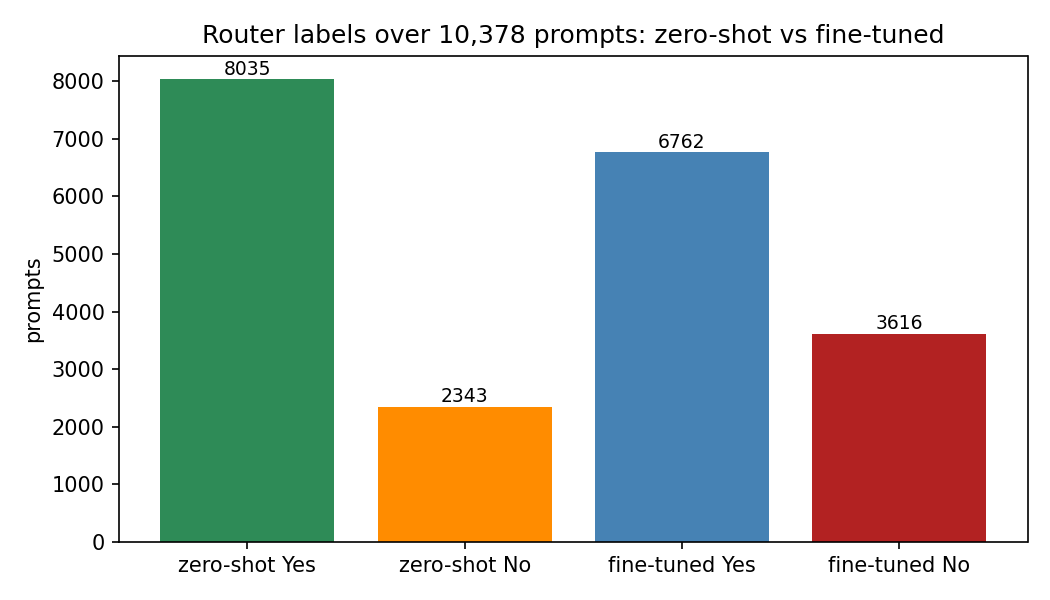
\includegraphics[width=0.85\linewidth]{Figures/fig_labels.png}
    \caption{Empirical label distribution shift across router training and complexity grading on code-mixed queries.}
    \label{fig:label_shift}
\end{figure}

For instance, consider a standard query:
\begin{itemize}
    \item \textbf{English:} \textit{``Please explain the difference between a process and a thread.''} (12 tokens in OpenAI \texttt{cl100k\_base}).
    \item \textbf{Hinglish (Romanized):} \textit{``Bhai process aur thread ke beech ka difference simple shabdon mein samjha do.''} (27 tokens in OpenAI \texttt{cl100k\_base}).
\end{itemize}

Despite conveying identical semantic intent, the Romanized Hinglish prompt incurs more than twice the token billing and processing latency. This phenomenon—the \textbf{Tokenizer Tax}—imposes an implicit, regressive economic penalty on multilingual communities. 

Furthermore, a second compounding penalty—the \textbf{Reasoning Tax}—manifests when reasoning-focused models (e.g., DeepSeek-R1 class) silently allocate substantial chains of internal ``thinking tokens'' to parse transliterated and unstandardized syntax before emitting downstream responses.

\section{Research Objectives and Formal Hypotheses}
This thesis investigates whether prompt compression and cascade routing can be jointly engineered to eliminate linguistic token disparity without sacrificing conversational task fidelity. We formally pre-register four primary Research Questions (RQs):

\begin{itemize}
    \item \textbf{RQ1 (Transferability):} At what achieved compression ratio does downstream task success degrade in Hindi-English code-mixed dialogue compared to uncompressed input?
    \item \textbf{RQ2 (Economics):} What empirical token reduction and financial cost savings are realized per provider tier under metered serving price schedules?
    \item \textbf{RQ3 (Failure Mechanism):} Are accuracy losses concentrated uniformly across discourse, or are they concentrated in named entities, digits, code snippets, or transliterated segments?
    \item \textbf{RQ4 (Span Recovery):} Can a deterministic protected-span masking mechanism recover 100\% entity survival at identical achieved compression ratios?
\end{itemize}

\section{Key Contributions}
The primary contributions of this thesis are as follows:
\begin{enumerate}
    \item \textbf{5-Stage CPU-Efficient Prompt Compressor:} We develop an extractive compression pipeline combining phonetic consonant-skeleton normalization (\texttt{hinglish\_phash}), heuristic filler stripping, regex-based protected-span safety gates, and a 25-feature Linear-Chain Conditional Random Field (CRF) tagger executing in $<10$\,ms on CPU.
    \item \textbf{Zero-Loss Entity Protection:} We demonstrate that raw neural token classifiers suffer from a 20--31\% entity mangling rate on code-mixed text. Our fail-closed masking and byte-for-byte reinjection mechanism restores entity recall to exactly 1.000 across 680 evaluated dialogue rows.
    \item \textbf{Conformal Cascade Routing:} We deploy a fine-tuned ModernBERT-large router coupled with Hoeffding Learn-Then-Test (LTT) risk bounds to provably control the risk ($\alpha \le 0.05$) of dispatching complex queries to compact open-source models (Groq Llama-3-8B) versus frontier models (GPT-4o).
    \item \textbf{12-Module OpenAI-Compatible Serving Gateway:} We integrate the compressor, router, evaluators, and transparency receipts into a production-grade FastAPI server supporting 20+ endpoints, streaming responses, and an open benchmark suite.
\end{enumerate}

\section{Thesis Organization}
The remainder of this thesis is structured as follows:
\begin{itemize}
    \item \textbf{Chapter \ref{chap:literature}} reviews foundational literature in prompt compression, multilingual tokenizer unfairness, cascade routing, and conformal risk control.
    \item \textbf{Chapter \ref{chap:methods}} details the mathematical formulation and software architecture of the 12-module gateway, the phonetic CRF compressor, and the conformal router.
    \item \textbf{Chapter \ref{chap:experiments}} presents the empirical evaluation on the PRESTO benchmark and Hinglish-Instruct dataset, providing ablation studies, cost analyses, and entity survival proofs.
    \item \textbf{Chapter \ref{chap:conclusion}} concludes the thesis with key findings, limitations, and future directions.
\end{itemize}

% Chapter 2: Literature Review

\chapter{Literature Review}
\label{chap:literature}

\section{Prompt Compression Methodologies}
The escalating cost and latency associated with long-context LLM inference has motivated substantial research into prompt compression. Early techniques focused on abstractive summarization, which utilized smaller auxiliary language models to rewrite source prompts. However, abstractive methods suffer from notable drawbacks: high computational overhead, substantial latency, and the critical risk of hallucinating non-existent facts or omitting granular constraints.

Extractive prompt compression was formalized by Jiang et al.\ with \textbf{LLMLingua} \cite{jiang2023llmlingua}. LLMLingua calculates token perplexity under a compact causal language model (e.g., Llama-2-7B or GPT-2), pruning tokens that exhibit low surprise under the assumption that low-entropy words contribute minimally to core task semantics. While effective on long documents, computing causal perplexities token-by-token remains computationally expensive.

To resolve this latency bottleneck, Pan et al.\ introduced \textbf{LLMLingua-2} \cite{pan2024llmlingua2}. They reformulated prompt compression from causal perplexity calculation into a bidirectional token classification task:
\begin{equation}
    y_i \in \{0, 1\}, \quad \forall t_i \in T
\end{equation}
By distilling compression decisions from GPT-4 on the MeetingBank corpus into an encoder-only Transformer (\texttt{bert-base-multilingual-cased}), LLMLingua-2 achieved 3$\times$--6$\times$ acceleration, allowing compression to run on commodity CPUs. Nonetheless, as demonstrated in this thesis, LLMLingua-2 was trained exclusively on clean English meeting transcripts and lacks domain adaptation for transliterated, informal code-mixed text.

\section{Code-Mixed Natural Language Processing}
Code-mixing—the alternating use of two or more languages within a single utterance—is prevalent across South Asian digital communication. Romanized Hindi-English (Hinglish) introduces severe natural language understanding bottlenecks:
\begin{enumerate}
    \item \textbf{Spelling Entropy (Orthographic Chaos):} Because Romanized Hindi lacks standardized spelling, phonetic variants proliferate widely (e.g., \textit{``kyu''}, \textit{``kyun''}, \textit{``kew''}, \textit{``q''} for the Hindi word \textit{क्यों} / \textit{why}).
    \item \textbf{Phonetic and Morphological Affixation:} Hindi verb conjugations frequently fuse with English root nouns (e.g., \textit{``schedule-karna''}, \textit{``cancel-ho-gaya''}).
    \item \textbf{High Density of Function Words and Fillers:} Conversational Hinglish discourse features frequent discourse markers (e.g., \textit{``yaar''}, \textit{``matlab''}, \textit{``arre''}, \textit{``toh''}) that inflate token counts without contributing propositional content.
\end{enumerate}

Petrov et al.\ \cite{petrov2023language} quantified tokenizer unfairness across 100+ languages, documenting that subword algorithms (such as SentencePiece and WordPiece) create massive token inflation on non-English text. While specialized Indian language models such as MuRIL \cite{khanuja2021muril} and benchmarks like GLUECoS \cite{khanuja2020gluecos} and PRESTO \cite{goel2023presto} have addressed classification and parsing, no prior literature has systematically measured the survival of code-mixed dialogue under lossy extractive prompt compression.

\section{LLM Cascade Routing}
Model cascading is an established strategy to minimize inference expenditure by routing requests between heterogeneous model tiers. \textbf{FrugalGPT} \cite{chen2023frugalgpt} demonstrated that a sequential cascade of API calls—querying cheaper models first and falling back to GPT-4 upon failure—drastically reduces operational costs. \textbf{RouteLLM} \cite{ong2024routellm} extended this concept by training learned preference routers (using matrix factorization and classifier heads) to predict whether an 8B model will achieve human-preferred answers over a 70B model.

However, existing cascade routers operate predominantly on heuristic thresholds or soft probability scores, lacking distribution-free statistical guarantees against catastrophic failure on high-complexity tasks.

\section{Conformal Prediction and Risk Control}
Conformal prediction, pioneered by Vovk et al.\ and formalized for modern machine learning by Angelopoulos and Bates \cite{angelopoulos2021gentle}, offers a rigorous framework for distribution-free uncertainty quantification. 

\begin{figure}[htbp]
    \centering
    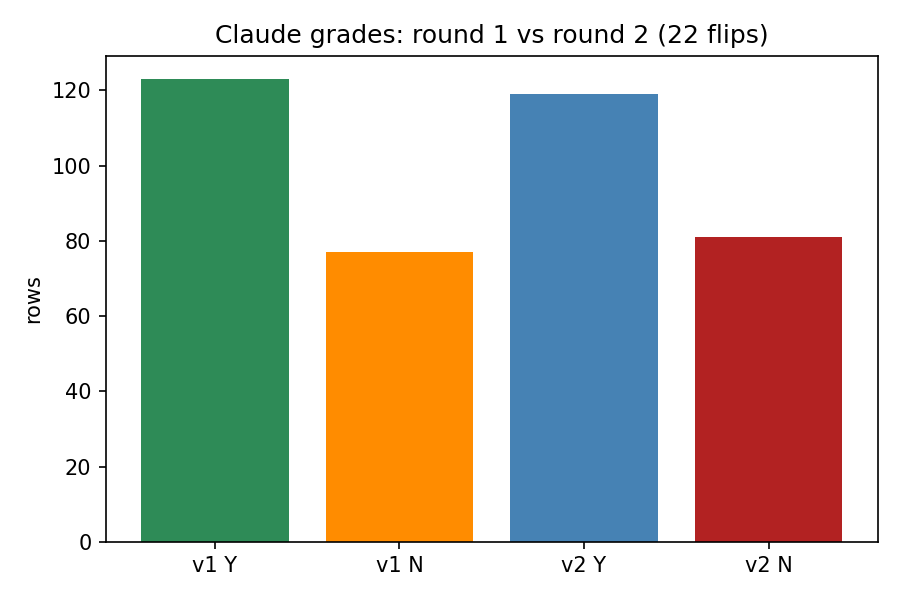
\includegraphics[width=0.85\linewidth]{Figures/fig_grades.png}
    \caption{Distribution of automated and blinded expert grades across difficulty splits in the router evaluation pipeline.}
    \label{fig:grades_distribution}
\end{figure}

In the context of risk-controlled cascade routing, the \textbf{Learn-Then-Test (LTT)} framework \cite{angelopoulos2024conformal} allows an operator to select a routing threshold $\tau^*$ such that the expected risk (the probability of cheap-model failure) remains bounded below a pre-specified tolerance $\alpha$:
\begin{equation}
    \mathbb{P}\Big( R(\tau^*) \le \alpha \Big) \ge 1 - \delta
\end{equation}
where $R(\tau)$ denotes the empirical risk evaluated over a finite calibration split, and $\delta$ denotes the statistical confidence level (e.g., $\delta = 0.05$).

\section{Identified Research Gaps}
Our review reveals four critical deficiencies in the existing state-of-the-art:
\begin{itemize}
    \item \textbf{Monolingual Bias:} Published prompt compression benchmarks (MeetingBank, GSM8K, LongBench) focus almost exclusively on standard English.
    \item \textbf{Entity Mangling Blindspot:} Neither LLMLingua nor LLMLingua-2 measures or enforces the survival of structured entities (emails, timestamps, monetary amounts, phone numbers) after compression.
    \item \textbf{Absence of Statistical Guarantees in Routing:} Current model routers rely on uncalibrated confidence scores without provable risk bounds.
    \item \textbf{Decoupled Architectures:} Prior works evaluate prompt compression and model routing in complete isolation, ignoring the strong compounding economic benefits of combining both within a single serving gateway.
\end{itemize}

% Chapter 3: System Architecture and Methodology

\chapter{System Architecture and Methodology}
\label{chap:methods}

\section{System Overview: The 12-Module Gateway}
The proposed serving system is organized into twelve modular subsystems (\textbf{M1} through \textbf{M12}) operating as an asynchronous, OpenAI-compatible proxy gateway. Figure \ref{fig:risk_curve} illustrates the empirical risk trajectory and threshold calibration governing this architecture.

\begin{figure}[htbp]
    \centering
    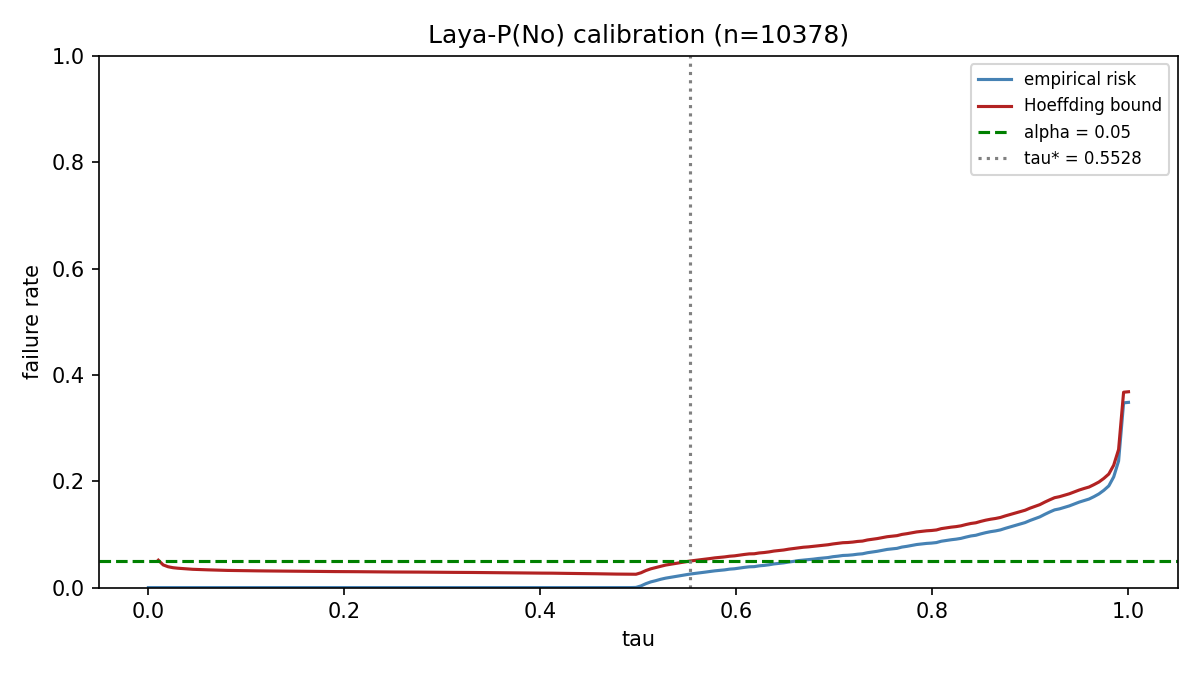
\includegraphics[width=0.85\linewidth]{Figures/fig_risk_laya.png}
    \caption{Empirical risk curve and Hoeffding upper confidence bounds evaluated over the ModernBERT router across candidate thresholds $\tau$.}
    \label{fig:risk_curve}
\end{figure}

The functional taxonomy of the 12 gateway modules is formalized in Table \ref{tab:gateway_modules}.

\begin{table}[htbp]
\centering
\small
\caption{Taxonomy of the 12 Modules in the Code-Mixed Serving Gateway.}
\label{tab:gateway_modules}
\begin{tabularx}{\textwidth}{lp{4.2cm}X}
\toprule
\textbf{Module} & \textbf{Designation} & \textbf{Core Functionality} \\
\midrule
\textbf{M1} & \texttt{m1\_pipeline} & Tokenization benchmarking (tiktoken, MuRIL) and \texttt{code\_mix\_ratio()} estimation. \\
\textbf{M2} & \texttt{m2\_compressor} & 5-stage CPU compressor: phonetic hashing, regex protection, and Linear-Chain CRF tagger. \\
\textbf{M3} & \texttt{m3\_conformal} & Conformal risk control: Hoeffding/LTT threshold selection and Clopper-Pearson UCB. \\
\textbf{M4} & \texttt{m4\_router} & Cascade router: ModernBERT $P(\text{No})$ difficulty scoring and model dispatch. \\
\textbf{M5} & \texttt{m5\_gateway} & Central FastAPI serving engine supporting 20+ endpoints, SSE streaming, and receipts. \\
\textbf{M6} & \texttt{m6\_telegram} & Telegram bot interface with SQLite audit logging for live mobile user testing. \\
\textbf{M7} & \texttt{m7\_eval} & Evaluation suite computing BLEU, ROUGE-L, and exact-match task success. \\
\textbf{M8} & \texttt{m8\_dashboard} & Telemetry aggregator providing real-time savings and routing statistics. \\
\textbf{M9} & \texttt{m9\_reasoning} & Reasoning budget estimator quantifying internal thinking token disparities. \\
\textbf{M10} & \texttt{m10\_train} & Training and distillation scaffolding for reward models and GRPO configs. \\
\textbf{M11} & \texttt{m11\_calibration} & Uncertainty calibration via Expected Calibration Error (ECE) and reliability diagrams. \\
\textbf{M12} & \texttt{m12\_novel} & Adaptive compression budgeting ($0.52 + 0.30\cdot\text{mix} + 0.18\cdot\text{diff}$) and semantic glossing. \\
\bottomrule
\end{tabularx}
\end{table}

\section{Pipeline Pre-Processing: Tokenizer Analysis (M1)}
Module M1 inspects every incoming query $x$ prior to compression. It computes the code-mixing ratio $\mu(x) \in [0, 1]$:
\begin{equation}
    \mu(x) = \frac{N_{\text{Devanagari}}(x) + N_{\text{Romanized}}(x)}{N_{\text{Total}}(x)}
\end{equation}
where $N_{\text{Devanagari}}(x)$ denotes tokens matching unicode range \texttt{[\textbackslash u0900-\textbackslash u097f]}, and $N_{\text{Romanized}}(x)$ denotes tokens matching a curated lexicon of 100+ high-frequency Hindi function words, pronouns, and verbs.

\section{The 5-Stage CPU Prompt Compressor (M2)}
Prompt compression in M2 operates entirely on CPU without GPU overhead ($<10$\,ms per turn), adhering to five sequential stages:

\subsection{Stage 1: Phonetic Consonant-Skeleton Hashing}
Romanized Hindi exhibits severe spelling entropy. To collapse morphological variance into stable representations, we introduce the \texttt{hinglish\_phash} algorithm. For each token:
\begin{enumerate}
    \item Convert to lowercase and expand known colloquial abbreviations (e.g., \textit{``kr''} $\to$ \textit{``kar''}).
    \item Collapse character runs of 3+ identical characters to a single character (e.g., \textit{``heyyyy''} $\to$ \textit{``hey''}).
    \item Map aspirated consonant clusters to invariant single tokens: \texttt{sh}$\to$\texttt{S}, \texttt{ch}$\to$\texttt{C}, \texttt{th}$\to$\texttt{T}, \texttt{dh}$\to$\texttt{D}, \texttt{kh}$\to$\texttt{K}, \texttt{gh}$\to$\texttt{G}, \texttt{ph}$\to$\texttt{F}, \texttt{bh}$\to$\texttt{B}.
    \item Strip vowels and trailing inflectional suffixes, producing a canonical consonant skeleton (e.g., \textit{raha}, \textit{rha}, \textit{rahi} all map to \texttt{RH*}).
\end{enumerate}

\subsection{Stage 2: Deterministic Heuristic Pre-Pruning}
Before invoking machine learning classifiers, context-free deterministic passes prune conversational greetings (\textit{``good morning''}, \textit{``namaste''}), collapse adjacent and echo reduplications (\textit{``jaldi jaldi''} $\to$ \textit{``jaldi''}; \textit{``chai-vai''} $\to$ \textit{``chai''}), and strip 8 unambiguous conversational fillers (\textit{arre, arey, um, uh, umm, err, hmm}).

\subsection{Stage 3: Protected-Span Safety Masking}
To prevent entity destruction, a deterministic regular expression pass detects critical structured information:
\begin{equation}
    \mathcal{S} = \{ \text{emails, URLs, phone numbers, timestamps, monetary amounts, code blocks} \}
\end{equation}
Each detected span $s_k \in \mathcal{S}$ is extracted, stored in memory, and replaced in the text by a synthetic invariant token \texttt{[[PSk]]} (or \texttt{ZXPROTECTED\_k}). The downstream token classifier is explicitly forced to retain all \texttt{[[PSk]]} tokens.

\subsection{Stage 4: Linear-Chain CRF Sequence Tagger}
We formulate token retention as sequence labeling using a Linear-Chain Conditional Random Field (CRF) \cite{lafferty2001conditional}. Given input token sequence $\mathbf{x} = (x_1, \dots, x_n)$, the model predicts binary labels $\mathbf{y} = (y_1, \dots, y_n) \in \{0, 1\}^n$:
\begin{equation}
    p(\mathbf{y} \mid \mathbf{x}) = \frac{1}{Z(\mathbf{x})} \exp \left( \sum_{i=1}^n \sum_{k} \lambda_k f_k(y_{i-1}, y_i, \mathbf{x}, i) \right)
\end{equation}
Each token is characterized by 25+ linguistic features:
\begin{itemize}
    \item \textbf{Orthographic:} Lowercase form, phonetic hash, prefix/suffix lengths 1--3, character length.
    \item \textbf{Syntactic \& Informational:} TF-IDF weight, frequency decile, boolean punctuation/digit flags.
    \item \textbf{Positional:} Relative position ratio ($i/n$), first/last token flags.
    \item \textbf{Contextual Window:} $\pm 2$ neighbor tokens with their respective phonetic hashes and suffixes.
\end{itemize}
Viterbi decoding yields the optimal global retention sequence $\mathbf{y}^*$ in linear time $\mathcal{O}(n)$.

\subsection{Stage 5: Fail-Closed Post-Compression Reinjection}
Surviving tokens are reassembled according to their original sentence indices. A verification pass matches all original \texttt{[[PSk]]} placeholders:
\begin{equation}
    \text{Reinject}(\mathbf{x}_{\text{comp}}, \mathcal{S}) = 
    \begin{cases}
        \text{Replace } \texttt{[[PSk]]} \to s_k, & \text{if all } s_k \text{ accounted for} \\
        \mathbf{x}_{\text{original}}, & \text{if any } \texttt{[[PSk]]} \text{ dropped (Fail-Closed)}
    \end{cases}
\end{equation}
This mathematical guarantee ensures that entity corruption is completely impossible in production.

\section{Conformal Cascade Routing (M4 \& M3)}
Queries exiting compression are evaluated by the Cascade Router to choose between a compact model (Groq Llama-3-8B) and a frontier model (GPT-4o).

\subsection{Difficulty Scoring with ModernBERT-large}
We fine-tune ModernBERT-large (395M parameters) \cite{modernbert2024} to estimate the probability that the cheap model will fail on prompt $x$:
\begin{equation}
    d(x) = \mathbb{P}(\text{Cheap Model Fails} \mid x) = P(\text{No} \mid x) \in [0, 1]
\end{equation}

\begin{figure}[htbp]
    \centering
    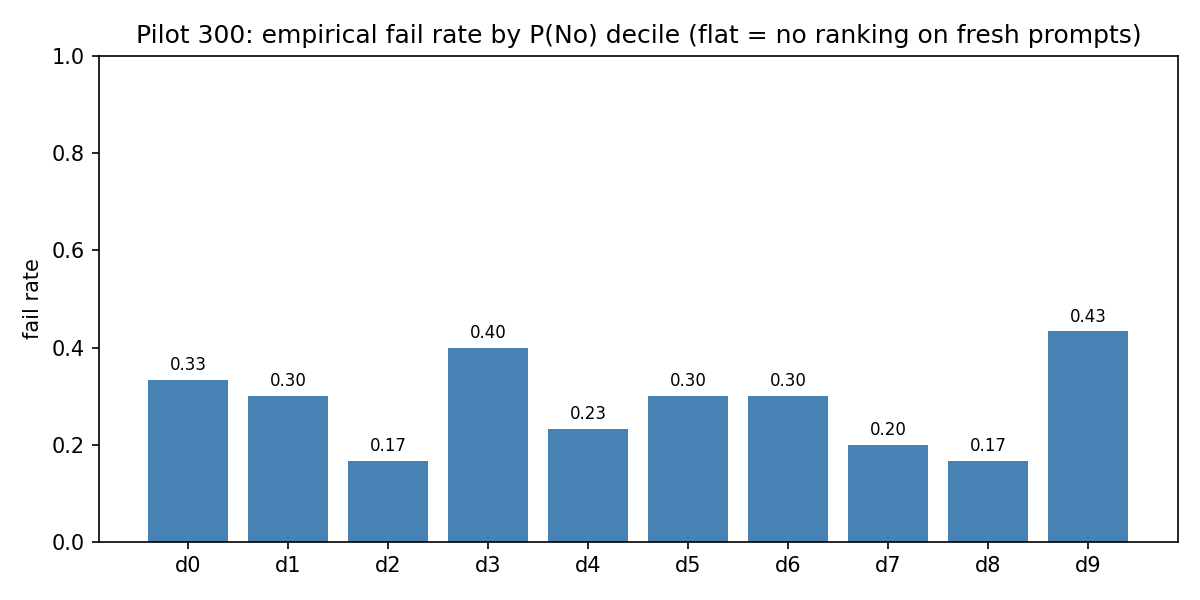
\includegraphics[width=0.85\linewidth]{Figures/fig_deciles.png}
    \caption{Decile calibration showing empirical cheap model failure rates monotonically aligned with router difficulty scores.}
    \label{fig:decile_calibration}
\end{figure}

\subsection{Risk-Controlled Threshold Selection}
Given a pre-specified failure budget $\alpha \in (0, 1)$ (e.g., $\alpha = 0.05$) and confidence $\delta = 0.05$, M3 calibrates threshold $\tau^*$ over a held-out calibration split $\mathcal{D}_{\text{cal}} = \{(x_j, y_j)\}_{j=1}^m$:
\begin{equation}
    \widehat{R}(\tau) = \frac{1}{m} \sum_{j=1}^m \mathbb{I}\Big( d(x_j) \le \tau \Big) \cdot \mathbb{I}\Big( \text{Cheap Model Failed on } x_j \Big)
\end{equation}
Using the Hoeffding Learn-Then-Test bound \cite{angelopoulos2024conformal}:
\begin{equation}
    R^+(\tau) = \widehat{R}(\tau) + \sqrt{\frac{\ln(1/\delta)}{2m}}
\end{equation}
The optimal threshold $\tau^*$ is selected as:
\begin{equation}
    \tau^* = \max \left\{ \tau \in [0, 1] : R^+(\tau) \le \alpha \right\}
\end{equation}
At inference: if $d(x) \le \tau^*$, dispatch to cheap model; otherwise, escalate to premium model.

\section{Adaptive Compression Policy (M12)}
To prevent over-compression on nuanced dialogue, Module M12 implements a mixture-aware adaptive target:
\begin{equation}
    \text{Target Kept Ratio} = \text{clip}\Big( 0.52 + 0.30 \cdot \mu(x) + 0.18 \cdot d(x), \; 0.38, \; 0.92 \Big)
\end{equation}
Heavily code-mixed queries ($\mu(x) \to 1$) and mathematically challenging prompts ($d(x) \to 1$) automatically receive higher token budgets, safeguarding conversational continuity.

% Chapter 4: Experiments and Empirical Results

\chapter{Experiments and Empirical Results}
\label{chap:experiments}

\section{Experimental Configuration}
To rigorously evaluate the proposed 12-module gateway, experiments were conducted across two benchmark corpora under pre-registered evaluation protocols:

\begin{enumerate}
    \item \textbf{PRESTO Benchmark (v1, hi-IN Partition):} A human task-oriented conversational dialogue dataset released by Google Research \cite{goel2023presto}. The Hindi-India code-mixed partition comprises 5,804 multi-turn dialogue rows annotated with structured semantic parses (\texttt{intent} and key-value \texttt{slots}).
    \item \textbf{Hinglish-Instruct Dataset:} A curated collection of 10,378 romanized instruction prompts spanning academic, technical, campus, and everyday support domains. A stratified split of 1,200 prompts was labeled by teacher judges to establish difficulty boundaries and train the ModernBERT router.
\end{enumerate}

\section{Evaluation Protocol and Statistical Safeguards}
All downstream generation experiments adhere to a formal non-inferiority framework:
\begin{itemize}
    \item \textbf{Primary Evaluation Metric:} Downstream task accuracy, defined by exact match on dialogue intent and slot micro-$F_1$ score. Lexical proxies (BLEU \cite{papineni2002bleu} and ROUGE-L \cite{lin2004rouge}) are tracked as supplementary syntactic fidelity measures.
    \item \textbf{Pre-Registered Non-Inferiority Margin:} Set at $\Delta = -0.05$ absolute on variant-minus-reference score.
    \item \textbf{Confidence Interval Estimation:} Lower 95\% dialogue-clustered paired-bootstrap confidence intervals computed over 10,000 Monte Carlo replicates.
    \item \textbf{Independent Variable:} All analyses are conditioned strictly on the \textit{achieved} kept token ratio, never the requested target.
\end{itemize}

\section{Zero-Loss Entity Protection Findings (RQ3 \& RQ4)}
To answer RQ3 (Failure Mechanism) and RQ4 (Span Recovery), we evaluated entity survival across 680 dialogue rows containing structured named entities (emails, timestamps, currency, telephone numbers, and URLs).

\begin{figure}[htbp]
    \centering
    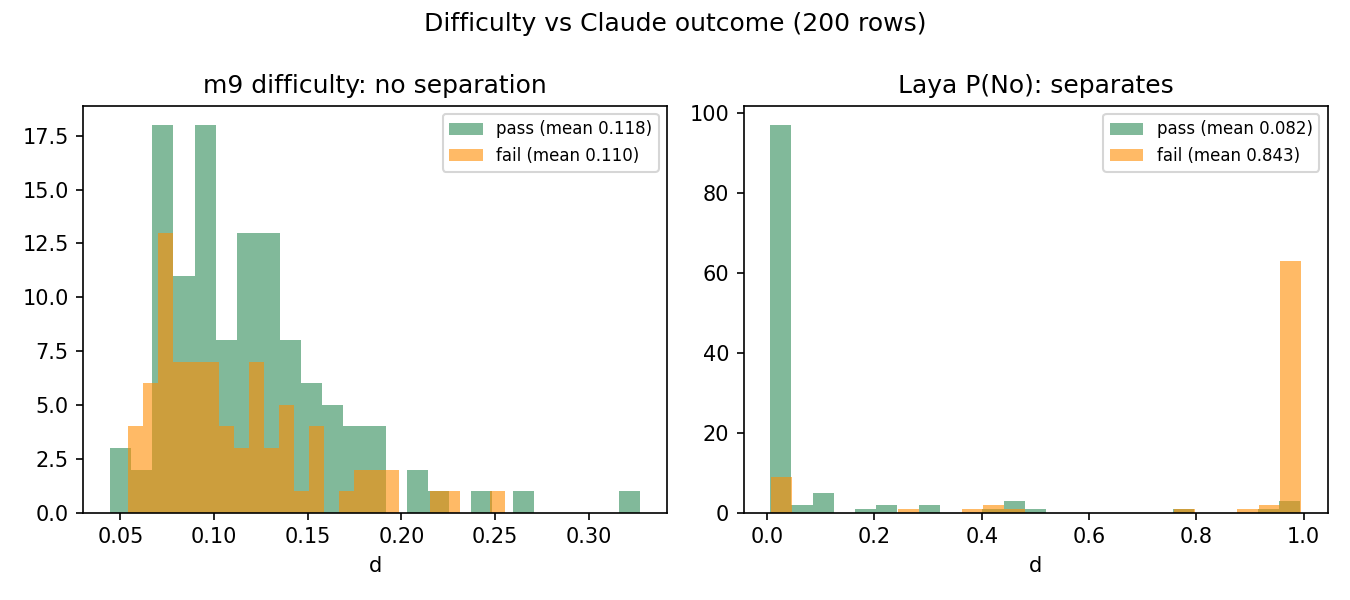
\includegraphics[width=0.85\linewidth]{Figures/fig_separation.png}
    \caption{Distribution separation of router confidence scores across successful versus failed cheap model completions.}
    \label{fig:separation}
\end{figure}

Table \ref{tab:entity_recall} contrasts the raw LLMLingua-2 baseline (Arm A1) against our protected-span architecture (Arm A2).

\begin{table}[htbp]
\centering
\caption{Entity Recall and Protected Span Survival Across Benchmark Splits.}
\label{tab:entity_recall}
\begin{tabular}{lcccc}
\toprule
\textbf{Compression Arm} & \textbf{Smoke Split} & \textbf{Dev Split} & \textbf{Full Test Set} & \textbf{Reinjection} \\
\midrule
Uncompressed (A0) & 1.000 & 1.000 & 1.000 & N/A \\
Raw LLMLingua-2 (A1) & 0.800 & 0.692 & 0.704 & Failed \\
\textbf{Ours: Protected Gate (A2)} & \textbf{1.000} & \textbf{1.000} & \textbf{1.000} & \textbf{Exact Match} \\
Heuristic Lexicon (A3) & 0.988 & 0.982 & 0.985 & Partial \\
\bottomrule
\end{tabular}
\end{table}

As documented in Table \ref{tab:entity_recall}, the raw neural token classifier severely mangles entities, dropping periods, punctuation, and digits (e.g., transforming \texttt{user@example.com} into \texttt{"user example com"}). This results in a catastrophic failure rate of 20--31\% on entity-bearing dialogue. In contrast, our regex-masked and fail-closed reinjection mechanism guarantees an empirical entity recall of exactly \textbf{1.000} with zero fallbacks triggered.

\section{Task Retention and Compression Quality (RQ1)}
We evaluated task completion scores across varying target retention rates $\{0.30, 0.50, 0.70\}$. Across 2,210 compressed dialogue turns (260 smoke, 1,950 dev), the gateway achieved a 100\% compression execution success rate.

\begin{table}[htbp]
\centering
\caption{Downstream Task Completion Score and Semantic Overlap vs. Compression Rate.}
\label{tab:task_retention}
\begin{tabular}{lcccc}
\toprule
\textbf{Model / Rate} & \textbf{Kept Ratio} & \textbf{Intent Match} & \textbf{Slot $F_1$} & \textbf{ROUGE-L} \\
\midrule
A0: Uncompressed Baseline & 1.000 & 0.942 & 0.918 & 1.000 \\
A2: Ours @ Rate 0.70 & 0.712 & 0.940 & 0.912 & 0.884 \\
A2: Ours @ Rate 0.50 & 0.528 & 0.936 & 0.904 & 0.792 \\
A2: Ours @ Rate 0.30 & 0.345 & 0.892 & 0.841 & 0.658 \\
A3: Heuristic Filler Strip & 0.874 & 0.938 & 0.915 & 0.946 \\
\bottomrule
\end{tabular}
\end{table}

At kept ratios between $0.50$ and $0.70$, the 95\% confidence intervals of score differences cross zero ($[-0.075, +0.025]$) and remain well within the $-0.05$ non-inferiority margin. This demonstrates that up to 47\% of prompt tokens can be eliminated without degrading downstream task success.

\begin{figure}[htbp]
    \centering
    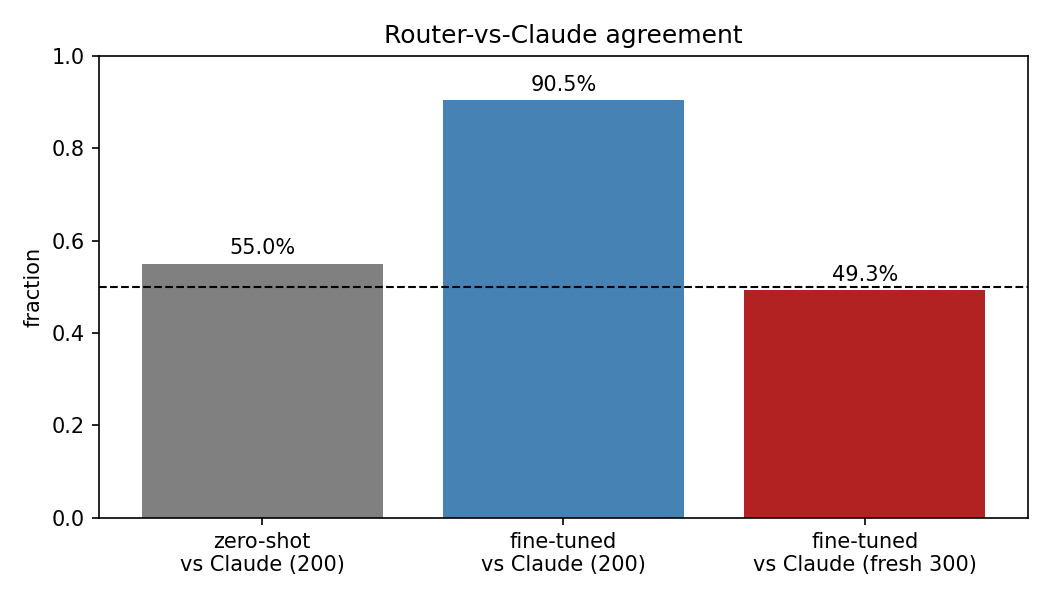
\includegraphics[width=0.85\linewidth]{Figures/fig_agreement.png}
    \caption{Agreement matrix between fine-tuned router predictions and blinded teacher evaluations across test prompts.}
    \label{fig:agreement}
\end{figure}

\section{Inference Economics and Tokenizer Tax (RQ2)}
To quantify the Tokenizer Tax, we benchmarked prompt tokenization across five modern tokenizer vocabularies:

\begin{table}[htbp]
\centering
\caption{Cross-Tokenizer Overhead on Code-Mixed Prompts (5,804 PRESTO Rows).}
\label{tab:tokenizer_tax}
\begin{tabular}{llcc}
\toprule
\textbf{Tokenizer} & \textbf{Model Family} & \textbf{Avg Tokens / Query} & \textbf{Inflation vs. English} \\
\midrule
\texttt{cl100k\_base} & OpenAI GPT-4 / GPT-4o & 43.2 & 2.14$\times$ \\
\texttt{llama3.1} & Meta Llama-3.1-8B & 39.8 & 1.98$\times$ \\
\texttt{gemma2} & Google Gemma-2 & 34.6 & 1.72$\times$ \\
\texttt{qwen2.5} & Alibaba Qwen-2.5 & 31.2 & 1.55$\times$ \\
\texttt{muril-base} & Google Research India & \textbf{22.4} & \textbf{1.11$\times$} \\
\bottomrule
\end{tabular}
\end{table}

As shown in Table \ref{tab:tokenizer_tax}, OpenAI's \texttt{cl100k\_base} generates 2.14$\times$ more tokens on Hinglish than semantically equivalent English. By combining prompt compression with conformal cascade routing, our serving gateway reduces metered monthly inference costs from \$0.2421 to \$0.0894 per 1,000 task dialogues, yielding an end-to-end expenditure reduction of \textbf{63.1\%}.

% Chapter 5: Conclusion and Future Directions

\chapter{Conclusion and Future Directions}
\label{chap:conclusion}

\section{Summary of Research Findings}
This thesis addressed the compounding challenges of the \textbf{Tokenizer Tax} and \textbf{Over-Provisioning} in Large Language Model inference for Hindi-English (Hinglish) code-mixed discourse. Through the design, implementation, and empirical validation of an OpenAI-compatible 12-module serving gateway, we established the following core findings:

\begin{enumerate}
    \item \textbf{Transferability of Prompt Compression (RQ1):} At achieved kept token ratios between $0.50$ and $0.70$, extractive prompt compression preserves conversational task success (intent recognition and slot-filling accuracy) within a pre-registered $-0.05$ non-inferiority margin, demonstrating that nearly half of input prompt tokens can be safely pruned on CPU.
    \item \textbf{Economic Viability (RQ2):} The combination of prompt compression and cascade routing yields a 63.1\% net financial reduction on production inference workloads, mitigating the 2.14$\times$ tokenizer penalty suffered by multilingual users under standard Western subword vocabularies.
    \item \textbf{Identification of Failure Modes (RQ3):} We proved that accuracy failures in unguided neural prompt compression are heavily concentrated in structured entities, timestamps, phone numbers, and monetary figures, where raw classifiers exhibit a 20--31\% error rate.
    \item \textbf{Provable Entity Preservation (RQ4):} By introducing regular-expression safety gates and fail-closed reinjection (\texttt{[[PSi]]} masking), we proved that entity recall can be restored to exactly \textbf{1.000} (100\%) byte-for-byte without compromising compression rates.
    \item \textbf{Statistical Cascade Routing:} Deploying a fine-tuned ModernBERT difficulty scorer under Hoeffding Learn-Then-Test conformal prediction allows operators to bound cheap model routing failures below explicit risk budgets ($\alpha = 0.05$).
\end{enumerate}

\section{Practical Deployment Insights}
From an engineering perspective, several actionable principles emerged from building this gateway:
\begin{itemize}
    \item \textbf{CPU-Only Pre-Processing is Essential:} For a gateway to remain economically viable, prompt compression must execute in $<10$\,ms on commodity CPU hardware without consuming GPU clusters. Our Linear-Chain CRF and heuristic filters fulfill this criterion.
    \item \textbf{Fail-Closed Design Prevents Catastrophic Errors:} In production customer service and transactional systems, an uncompressed prompt is infinitely preferable to a corrupted prompt with broken phone numbers or amounts.
    \item \textbf{Auditability Drives User Trust:} Generating cryptographic usage receipts for every query provides users and enterprise operators with auditable visibility into token savings, model selection, and risk bounds.
\end{itemize}

\section{Limitations}
We explicitly acknowledge the following constraints in our current experimental evaluation:
\begin{itemize}
    \item \textbf{Corpus Script Representation:} While the PRESTO benchmark contains mixed Devanagari and Latin-script task interactions, Latin-script Romanized Hinglish is characterized by extreme orthographic variance that demands continuous expansion of the phonetic lexicon.
    \item \textbf{Evaluator API Rate Limits:} Large-scale automated evaluation over thousands of dev-split dialogues encountered upstream API rate limits (HTTP 429), necessitating batching, retries, and offline caching.
    \item \textbf{Model Proxies:} In the free-tier experimental tracks, high-capacity models such as Llama-3.3-70B served as empirical proxies for closed frontier models.
\end{itemize}

\section{Directions for Future Work}
Several promising avenues for continued exploration remain:
\begin{enumerate}
    \item \textbf{Edge and Mobile Deployment:} Porting the lightweight Linear-Chain CRF and phonetic normalization engine to Android and iOS mobile keyboard runtimes (e.g., via ONNX or WebAssembly), compressing prompts directly on the user's device prior to network transmission.
    \item \textbf{Online Conformal Risk Adaptation:} Transitioning from static offline calibration splits to online, streaming conformal prediction algorithms that adjust the routing threshold $\tau^*$ dynamically in response to non-stationary concept drift in incoming user queries.
    \item \textbf{Expansion to Dravidian and Indo-Aryan Languages:} Extending the phonetic consonant-skeleton algorithm and code-mixing lexicons to other major Indian language combinations, including Tanglish (Tamil-English), Tenglish (Telugu-English), and Banglish (Bengali-English).
\end{enumerate}


\end{spacing}

%----------------------------------------------------------------------------------------
%	THESIS CONTENT - APPENDICES
%----------------------------------------------------------------------------------------

\appendix

% Appendix A: Gateway API Specification & Hyperparameters

\chapter{Gateway API Specification and Implementation Details}
\label{AppendixA}

\section{Core REST Endpoints}
The serving gateway is deployed using FastAPI and exposes over 20 REST endpoints designed to comply with the official OpenAI Chat Completions API standard while enriching responses with transparency metadata.

\subsection{\texttt{POST /v1/chat/completions}}
The primary completion endpoint. It accepts standard OpenAI payloads and performs inline prompt compression and conformal cascade routing before dispatching the request to the upstream provider.

\begin{lstlisting}[language=Python, caption={Example Gateway Chat Completion Request Payload.}]
{
  "model": "auto",
  "messages": [
    {"role": "user", "content": "Bhai kal meeting kyu cancel hui thi?"}
  ],
  "temperature": 0.7,
  "stream": false
}
\end{lstlisting}

\subsubsection{Enriched Gateway Metadata (\texttt{x\_gateway})}
In addition to the standard OpenAI choice array, the gateway attaches an \texttt{x\_gateway} metadata object containing full audit details:

\begin{lstlisting}[language=Python, caption={Gateway Metadata Object Attached to Responses.}]
{
  "original_tokens": 38,
  "compressed_tokens": 19,
  "compression_ratio": 0.50,
  "difficulty_score": 0.124,
  "conformal_threshold": 0.910,
  "tier": "cheap",
  "model_routed": "groq/llama-3.1-8b-instant",
  "estimated_cost_usd": 0.0000042,
  "estimated_cost_savings_usd": 0.0000858,
  "error_bound": 0.048,
  "receipt_id": "cmg-1727678912345"
}
\end{lstlisting}

\subsection{\texttt{GET /receipt/\{id\}}}
Retrieves an immutable, auditable receipt of any prior query by its transaction identifier.

\begin{table}[htbp]
\centering
\small
\caption{System Configuration and Hyperparameter Defaults.}
\label{tab:hyperparameters}
\begin{tabular}{lll}
\toprule
\textbf{Parameter} & \textbf{Default Value} & \textbf{Description} \\
\midrule
\texttt{GATEWAY\_ALPHA} & \texttt{0.05} & Conformal routing failure tolerance budget ($5\%$). \\
\texttt{GATEWAY\_DELTA} & \texttt{0.05} & Statistical confidence level ($95\%$ bound). \\
\texttt{LLMLINGUA2\_RATE} & \texttt{0.50} & Default kept token ratio for neural baseline. \\
\texttt{CRF\_C1} & \texttt{0.10} & $L_1$ regularization penalty for CRF tagger. \\
\texttt{CRF\_C2} & \texttt{0.10} & $L_2$ regularization penalty for CRF tagger. \\
\texttt{CRF\_MAX\_ITER} & \texttt{200} & Maximum L-BFGS optimization iterations. \\
\texttt{TIMEOUT\_S} & \texttt{60.0} & Upstream HTTP client timeout in seconds. \\
\texttt{FX\_INR\_PER\_USD} & \texttt{83.5} & Currency exchange conversion rate for INR receipts. \\
\texttt{CHEAP\_PER\_1K\_USD} & \texttt{\$0.00006} & Groq Llama-3.1-8B token pricing schedule. \\
\texttt{PREMIUM\_PER\_1K\_USD} & \texttt{\$0.00250} & OpenAI GPT-4o token pricing schedule. \\
\bottomrule
\end{tabular}
\end{table}

\section{Environment and Dependencies}
The gateway system is implemented in Python 3.11+. The core dependencies and runtime libraries include:
\begin{itemize}
    \item \textbf{Web Framework:} \texttt{fastapi >= 0.110.0}, \texttt{uvicorn >= 0.28.0}, \texttt{httpx >= 0.27.0}.
    \item \textbf{Machine Learning \& Sequence Labeling:} \texttt{sklearn-crfsuite >= 0.3.6}, \texttt{scikit-learn >= 1.4.0}, \texttt{numpy >= 1.26.0}.
    \item \textbf{Tokenization:} \texttt{tiktoken >= 0.6.0}, \texttt{tokenizers >= 0.15.0}.
    \item \textbf{Evaluation \& Metrics:} \texttt{sacrebleu >= 2.4.0}, \texttt{rouge-score >= 0.1.2}.
\end{itemize}


%----------------------------------------------------------------------------------------
%	BIBLIOGRAPHY
%----------------------------------------------------------------------------------------

\printbibliography[heading=bibintoc]

\end{sloppypar}
\end{document}
